\documentclass[11pt]{article}

\usepackage{exscale}
\usepackage{graphicx}
\usepackage{amsmath}
\usepackage{latexsym}
\usepackage{times,mathptm}
\usepackage{epsfig}
\usepackage{setspace}

\textwidth 6.5truein          
\textheight 9.0truein
\oddsidemargin 0.0in
\topmargin -0.6in

\parindent 0pt          
\parskip 5pt
\def\baselinestretch{1.1}

\begin{document}

\begin{LARGE}
\centerline {\bf CSci 423 Homework 6}
\end{LARGE}
\vskip 0.25cm

\centerline{Due: 1:00 pm, Wednesday, 10/24}
\centerline{Eric Shih}

\begin{enumerate}
  \item (10 points) Exercise 2.11 on page 129. \\
    \begin{center}
      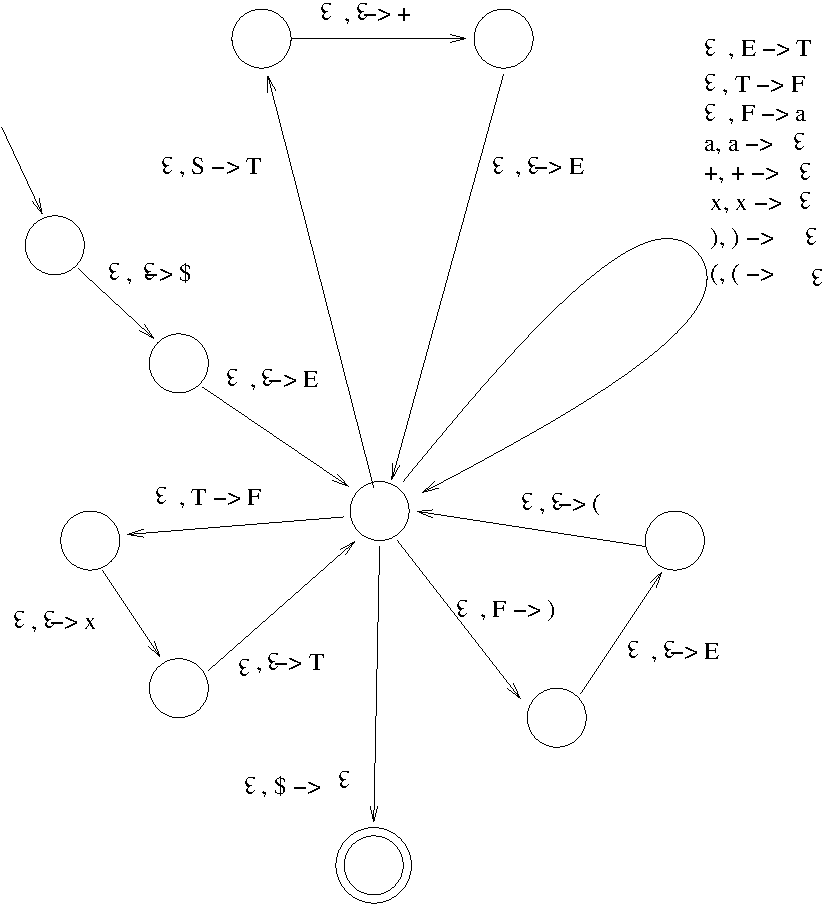
\includegraphics[scale=.7] {fig1.pdf}
    \end{center}
  \item (6 point) Problem 2.19 on page 130. \\
    $L(G)$ accepts all strings except $a^ib^i$. This means that the complement
    only accepts this string, thus the CFG for the complement of $L(G)$:
    \begin{center}
     $S \to aSb | \epsilon $
    \end{center}
  
  \item (6 points) Problem 2.21 on page 130. (No proof of correctness required) \\
    The CFG for $\Sigma$:
      \begin{center}
       $S \to aaSb | aSbSa | bSaa | SS | \epsilon $
      \end{center}

  \item (8 points) Problem 2.26 on page 130. \\
    First, the derivation involves the rules that follow the form $S \implies A_1A_2A_3 \dots A_n$.
    The derivation of $w$ will require $n-1$ uses of this type because a variable
    will need to be added for the increase in size. Second, the terminals being derived
    will take the for $S \implies a$. Thus because the $n$ number of derivations from
    each variable, $2n-1$ steps are required for any derivation of $w$.
    
  \item (10 points) Problem 2.24 on page 130. \\
    We use 3 cases to show that $E$ is context free.
    \begin{enumerate}
      \item $i < j $ \\
	    $S \to aSb | A $ \\
	    $A \to aA | a$
      \item $i<j<2i$ \\
	    $S \to aSb | aSbb | aabbb$
      \item $2i < j$ \\
	    $S \to aSbb|B $ \\
	    $B \to bB | b $
    \end{enumerate}

\end{enumerate}

\pagebreak
\setlength{\parindent}{1cm}
\centerline{\bf Reading Summary 3}

\begin{spacing}{1.5}
 Context free grammars were originally conceived as a way to describe natural languages. Since then, context
 free grammars have also been used to define many other concepts within Computer Science. Grammars have been used 
 to describe programming languages, namely, the act of turning a language description from a context free grammar
 into a parser. Another use of context free grammars can be seen in XML (Extensible Markup Language). Within XML 
 the Document Type Definition is a context free grammar that describes the allowable tags. These tags are familiar
 keywords from HTML, however these tags do no deal with formatting, but instead describe the meaning of the text.
 
 \indent Regular expressions are how programming languages are structured. However, there are also some aspects of 
 programming languages that cannot be represented using regular expressions. An example of this is the use of 
 parentheses in a nested fashion. Each set of parentheses must be matched correctly, which means that the grammars
 written must also follow this balance. In this case, CFGs can be used to easily show that a grammar is able to use
 parentheses, but also have them be balanced. The YACC parser-generator shows how CFGs can be used to parse languages.
 in this parser-generator, the input into the YACC is a CFG which runs through the machine that eventually generates
 fragments of C code in response to the parse tree.
 
 \indent In markup languages, tags are the strings that are used to give information about the semantics of various
 strings within the document. In the case of HTML, its major functions of creating links between documents and describing
 the format of a document use CFGs to describe and guide the process of a document. Tags always have a beginning form and
 sometimes have an end form. If there is not an end form, then the tags are usually matched at the end of a paragraph. A 
 CFG can be used to describe not only the syntax of HTML, but it can also be used to show the structure of the language. In
 more complex markup language, CFGs play a more important role. Document Type Definition is a CFG with its own notation,
 but the same principles for context-free grammars. It is essentially treated as a grammar that specifies to XML documents.
 Overall context-free grammars are a very useful application in a wide range of concepts.
\end{spacing}

\end{document}